\documentclass{article}
\usepackage[T1]{fontenc}
\usepackage{lmodern}
\usepackage{graphicx}
\usepackage{amsmath,amssymb}
\usepackage[a4paper,margin=2cm]{geometry}
\usepackage[absolute,overlay]{textpos}
\setlength{\TPHorizModule}{1mm}
\setlength{\TPVertModule}{1mm}
\usepackage[indonesian]{babel}
\usepackage{hyperref}
\setlength{\emergencystretch}{2em}
% unit: Halaman 33

\begin{document}

% === Halaman 33 (llm) ===

\begin{itemize}
    \item Contoh FSR adalah LFSR (\textit{Linear Feedback Shift Register})
\end{itemize}

\vspace{50mm}

\[ b_n = b_n \oplus b_{n-1} \oplus ... \oplus b_2 \oplus b_1 \]

\begin{itemize}
    \item Bit-bit di dalam register digeser satu bit ke kanan setiap kali pembangkitan bit luaran (= bit kunci alir atau \textit{keystream})
    \item Bit $b_n$ digeser ke tempat $b_{n-1}$, $b_{n-1}$ digeser ke $b_{n-2}$, dst, $b_2$ digeser ke $b_1$, $b_1$ terlempar ke luar
    \item Bit yang terlempar keluar ($b_1$) menjadi bit luaran LFSR
    \item Selanjutnya dihitung $b_n$ yang baru, yaitu $b_n = b_n \oplus b_{n-1} \oplus ... \oplus b_2 \oplus b_1$
\end{itemize}

% deskripsi: Diagram blok Register Geser (LFSR) yang menunjukkan pergeseran bit dari bn hingga b1 dengan jalur feedback menggunakan operasi XOR.
% bbox normalisasi: [0.1500, 0.1500, 0.7700, 0.4500]
\begin{textblock*}{130.20mm}(31.50mm,44.55mm)
\noindent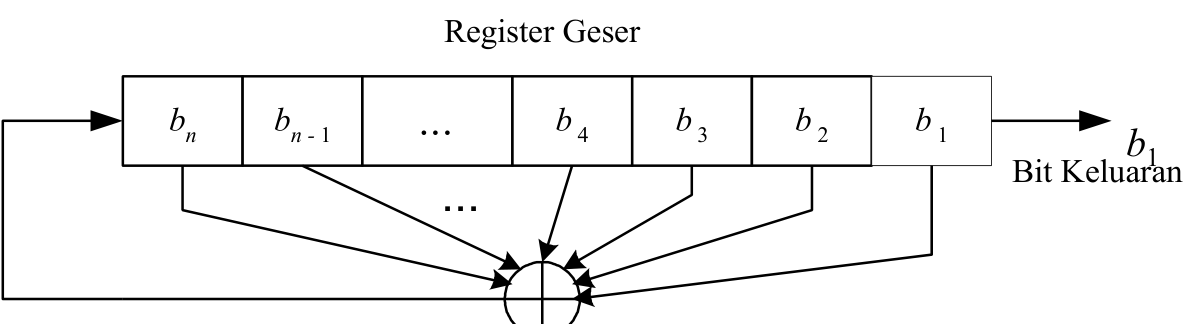
\includegraphics[width=130.20mm,height=89.10mm]{../../images/llm/page_033_img_01.png}%
\end{textblock*}

\end{document}
